\documentclass[journal,onecolumn,11pt]{IEEEtran} 
\ifCLASSINFOpdf
  % \usepackage[pdftex]{graphicx}
  % declare the path(s) where your graphic files are
  % \graphicspath{{../pdf/}{../jpeg/}}
  % and their extensions so you won't have to specify these with
  % every instance of \includegraphics
  % \DeclareGraphicsExtensions{.pdf,.jpeg,.png}
\else
  % or other class option (dvipsone, dvipdf, if not using dvips). graphicx
  % will default to the driver specified in the system graphics.cfg if no
  % driver is specified.
  % \usepackage[dvips]{graphicx}
  % declare the path(s) where your graphic files are
  % \graphicspath{{../eps/}}
  % and their extensions so you won't have to specify these with
  % every instance of \includegraphics
  % \DeclareGraphicsExtensions{.eps}
\fi

% packages added by fzen
\usepackage{graphicx}
\usepackage{sidecap}
\usepackage{xcolor}
\usepackage{glossaries}
\usepackage{comment}
\usepackage[margin=1.25in]{geometry}
\geometry{top=1in, left=1.25in, right=1.25in, bottom=1in}
\usepackage{setspace}
%\doublespacing
\usepackage[numbers, square, comma, sort&compress]{natbib}
\usepackage{caption}
\usepackage{mdframed}
\usepackage{subfig}
\DeclareCaptionType[fileext=box]{infobox}[Box]


\newcommand{\refeq}[1]{{Eq.~(\ref{#1})}}
\newcommand{\refeqs}[1]{{Eqs.~(\ref{#1})}}
\newcommand{\reffig}[1]{{\color{blue!70}(Fig.~\ref{#1})}}
\newcommand{\reftab}[1]{{\color{blue!70}(Tab.~\ref{#1})}}
\newcommand{\refbox}[1]{{\color{blue!70}(Box.~\ref{#1})}}
\newcommand{\reffigs}[1]{{Figs.~\ref{#1}}}
\newcommand{\refsec}[1]{{Sec.~\ref{#1}}}
\newcommand{\D}{\mathrm{d}}


% Define acronymns
% \makeglossary
\newacronym{sg}{SG}{surrogate gradient}
\newacronym{ann}{ANN}{artificial neural network}
\newacronym{rnn}{RNN}{recurrent neural network}
\newacronym{snn}{SNN}{spiking neural network}
\newacronym{stdp}{STDP}{spike timing-dependent plasticity}
\newacronym{bp}{BP}{back-propagation}
\newacronym{bptt}{BPTT}{back-propagation through time}
\newacronym{rtrl}{RTRL}{real-time recurrent learning}
\newacronym{lel}{LEL}{local error learning}
\newacronym{lif}{LIF}{leaky integrate-and-fire}
\newacronym{relu}{ReLU}{rectifying linear unit}
\newacronym{eRBP}{eRBP}{event-driven random back-propagation}
\newacronym{lstm}{LSTM}{long short-term memory}
\newcommand{\HM}[1]{\textcolor{red}{{\bf HM:}~#1}}

\begin{document}

\title{Learning to Solve Real-World Problems with Spiking Neural Networks}
% Other possible titles
% \title{Surrogate-gradient-descent learning in spiking neural networks}

\author{Emre O. Neftci$^\dagger$,~\IEEEmembership{Member,~IEEE,}
        Hesham Mostafa$^\dagger$,~\IEEEmembership{Member,~IEEE,}
        Friedemann Zenke$^\dagger$\\
        {\small $^\dagger$ All authors contributed equally. The order of authors is random.}}% <-this % stops a space
\markboth{IEEE SPM White Paper for the special issue on neuromorphic computing}%
{}
%
\maketitle
\IEEEpeerreviewmaketitle
%
\begin{abstract}
A growing number of neuromorphic \gls{snn} processors that emulate biological neural networks are creating an imminent need for methods and tools enabling them to solve real-world problems involving real-time signal processing.
Like conventional neural networks, \glspl{snn} are particularly efficient when trained on real, domain specific data. 
However, their training requires overcoming a number of challenges linked to their binary and dynamical nature.
This tutorial elucidates step-by-step the challenges typically encountered when training \glspl{snn}, and guides the reader through the key concepts of synaptic plasticity and data-driven learning in the spiking setting.
In so doing, it introduces surrogate gradient methods as a particularly flexible and efficient method to overcome the aforementioned challenges and discusses the ``tricks of the trade''. 
\end{abstract}


% I am adding this only to keep an overview during writing, fzenke
\tableofcontents
\newpage


\begin{center}
  * Shorten the introduction
  * Describe brain/spiking before the theoretical discussion on Turing machines.
  * Section V too long, breaks the flow. Move Alternative methods to box?
  
\end{center}

\section{Introduction}
%%I think we should start with brain inspiration. The special issue is about brain-inspires computing. 
%\textbf{Add "brain inspiration here"}
% TODO Add brain inspiration paragraph -- 20Watts etc ...  Signal processing
% introducing
A plethora of signal processing problems are concerned with real-time pattern recognition or noisy time series prediction.
%To solve real-world problems with intrinsically nonlinear dynamics and an inherent history dependence, 
\glspl{rnn} prove highly effective \cite{Goodfellow_etal16_deeplear} at solving such problems. 
% CITE review However, to deploy
%\textbf{motivation and brain inspiration}
\glspl{rnn} are a class of stateful neural networks whose internal state evolves either in continuous time or through discrete time steps.
%\begin{comment}
%  Emre: The Turing discussion is too detailed here. Make it briefer. Introduce brain-inspired/spiking earlier
%\end{comment}
%%Turing discussion, move to discussion?
%\glspl{rnn} are universal computing architectures that are able to reproduce the behavior of an arbitrary Turing machine~\cite{Siegelmann_Sontag95}.
%%% Following line can be deleted/moved.
%The {\it program} implemented by an \gls{rnn}, however, is described in a fundamentally different way from a conventional Turing machine.
%Instead of a state transition table or a sequence of instructions, the behavior of \gls{rnn} is implicitly defined by the network weights and the equations governing the behavior of each neuron in the network.
%While this implicit definition is harder to parse and understand than conventional programs, it makes it possible to learn by tuning the network weights.
%%
%Early on, Alan Turing recognized this potential of \glspl{rnn} in a prescient paper~\cite{Ince92} in which he described recurrent networks of logic gates where the connections between logic gates can be adapted to suit the task.
%Turing's paper was inspired by the most complex \glspl{rnn} known to us: biological brains.
While \glspl{rnn} used for practical applications nowadays are different in many fundamental ways from biological networks, they both share the same general architecture and employ learning based on weight adjustment.
%
The interest in \glspl{rnn} as a brain-inspired methods stems from a growing body of work is establishing formal equivalences between recurrent neural networks and a class of \glspl{snn} that can be efficiently emulated in dedicated neuromorphic hardware \cite{zenke_superspike:_2018,Wozniak_etal18_deepnetw,Neftci18_datapowe,Bellec_etal18_longshor}. 
It is thus natural to draw inspiration from biological networks for computing, as they were evolution's highly-optimized answer to the problem of sensory signal processing. 
\begin{comment}
  Emre: Merge the description of the training challenges with implementation challenges 
  Emre: Make the following discussoin more SNN-centric. What are the challenges of SNN
\end{comment}
\Glspl{rnn} and \Glspl{snn} are often trained using an optimization procedure in which the the parameters or weights are adjusted to minimize some objective function.
Training \Glspl{rnn} and \Glspl{snn} can be impeded by a variety of factors common for real world applications, e.g.\ noise and non-stationary of the data. 
% Overcoming these limitations is an active field of research, many of which
% have been reviewed in detail elsewhere CITE. % CITE find suitable review
As models grow larger and make their way into embedded and automotive applications, their power efficiency for both inference and training is of increasing importance \cite{boahen_neuromorphs_2017}. 
To tackle the latter problem, simplified neural network applications have been devised which are amenable to be run natively on dedicated hardware, such as neuromorphic hardware and neural network accelerators.  
For instance, one common approach are binary activation neural network implementations which can dispense with energetically costly floating-point multiplications. % CITE paper on binary embedded nets
These form a special subset of \glspl{rnn} with a binary activation functions and constitute a common ground between \Glspl{rnn} and \Glspl{snn}. 
%area of active study both due to their potential for power efficient computation and more fundamentally because \glspl{snn} are the dominant network model employed by the brain.

A body of work has focused on training spiking neural networks without hidden units \cite{ponulak_supervised_2009, Gutig_Sompolinsky06_tempneur,
florian_chronotron:_2012, mohemmed_span:_2012, memmesheimer_learning_2014, Anwani_Rajendran15_normappr}, \emph{i.e.}\ units which are neither directly connected to the input nor the output of the network.  
Properly training hidden units is necessary to solve a majority of complex, real-world problems.
Their training however requires efficient solutions to the spatial and temporal credit assignment problems, and creates a set of specific challenges.  

In this article we focus on these challenges and describe possible remedies by specifically considering the problem of supervised learning in \glspl{snn}.
%The two key challenges which need to be addressed to successfully train \glspl{snn} are concerned with the spatial and the temporal credit assignment,
%i.e.\ how weights and parameters of hidden units need to be modified to improve the objective during training.  
%
%\section{Types of \glspl{rnn}}
%{\bf Shouldn't we have a short section with a formal defintion first}
%Discrete-time RNN:
%\begin{align}
%x[n] = & \sigma(h[n]) \\
%h[n+1] = & f(h[n],{\bf W}x[n])
%\end{align}
%
%Continuous-time RNN
%\begin{align}
%x(t) = & \sigma(h(t)) \\
%\frac{dh}{dt} = &g(h(t),{\bf W}x(t))
%\end{align}
%
%Approximation of the continuous-time RNN by a discrete RNN
%
%\[
%\begin{split}
%x[t] = & \sigma(h[t]) \\
%h[t+1] = & h[t] + \Delta t g(h(t),{\bf W}x(t))
%\end{split}
%\]
%
%SNNs as binary RNNs (Friedman's part)

\section{Understanding \glspl{snn} as \glspl{rnn} (FRIEDEMANN)}
\label{sec:understanding_ssn_as_rnn}

In this section we provide a brief walk-through how to formally map a \gls{snn} to \gls{rnn} 
which will provide the basis to training a spiking neural network with \glspl{sg}.
To that end, we will first introduce the \gls{lif} neuron model
with current-based synapses as a standard neuron model which has wide use in computational neuroscience \cite{Gerstner_etal14_neurdyna}. 
Next, we will reformulate this model in discrete time and show its formal equivalence to a discrete time \gls{rnn} with binary activation function. 
Formulating \glspl{snn} as \glspl{rnn} 
allows us to directly transfer and apply existing methods to train \glspl{rnn} and will serve as the conceptional framework for the rest of this article. 
If you are not familiar with the \gls{lif} neuron model, you can skip most of the following derivations and up to Equation~\eqref{eq:mem_discrete_time}. 

% Introduce LIF in differential form
We begin by recalling that a single \gls{lif} neuron with index $i$ 
can formally be described in differential form as
\begin{equation}
    \tau_\mathrm{mem} \frac{\mathrm{d}U_i}{\mathrm{d}t} = -(U_i-U_\mathrm{rest}) + RI_i
    \label{eq:lif_basic}
\end{equation}
where $U_i(t)$ is the membrane potential which describes the state of the
neuron, $U_\mathrm{rest}$ is the resting potential, $\tau_\mathrm{mem}$ is the
membrane time constant, $R$ is the input resistance, and $I_i(t)$ is the 
input current \cite{Gerstner_etal14_neurdyna}.
It is easy to see that $U_i$ acts as a leaky integrator of the input current
$I_i$.
Strictly speaking Equation~\eqref{eq:lif_basic} only describes the subthreshold dynamics of a \gls{lif} neuron, i.e.\ the dynamics in absence of spiking output of the neuron.
Neurons emit spikes to communicate their output to other neurons when their membrane voltage hits the firing threshold $\vartheta$.
After each spike the membrane voltage $U_i$ is reset to the resting 
potential $U_i\rightarrow U_\mathrm{rest}$.

In spiking neural networks the input current is typically generated by synaptic
currents that are triggered by the arrival of presynaptic spikes $S_j(t)$.  When
working with differential equations, it is convenient to denote a spike train
$S_j$ as a sum of Dirac delta functions
$$S_j(t)=\sum_k \delta(t-t_j^k)$$
with the firing times $t_j^k$ of neuron $j$.
Where sensible and if not mentioned otherwise, we use the index variable $j$ for
presynaptic indices, whereas $i$ is reserved for postsynaptic neurons.

Synaptic currents are not static in time, but follow specific temporal dynamics
themselves. A reasonable first approximation is to model their time course as an
exponential current following each presynaptic spike. Moreover, we assume that
synaptic currents sum linearly. Thus we can write:
\begin{equation} 
    \frac{\mathrm{d}I_i}{\mathrm{d}t}= -\frac{I_i(t)}{\tau_\mathrm{syn}} + \sum_j W_j S_j(t)
    \label{eq:cuba_syn}
\end{equation}
where the sum runs over all presynaptic neurons $j$ and $W_j$ are the
afferent weights.  Neuron $i$ has an ``autapse'', ie.\ a self connection, if the
index $i$ appears in this sum.  Because of this property we can simulate a
single \gls{lif} neuron with two linear differential equations whose initial
conditions change instantaneously whenever a spike occurs.

By combining the above definitions into Equation~\eqref{eq:lif_basic} we get 
\begin{equation} 
    \frac{\mathrm{d}U_i}{\mathrm{d}t} = -\frac{1}{\tau_\mathrm{mem}}(U_i-U_\mathrm{rest}) + RI_i + S_i(t)(U_\mathrm{rest}-\vartheta)
    \label{eq:lif}
\end{equation}

% Formulate model in discrete time
It is customary to solve Equations~\eqref{eq:cuba_syn} and~\eqref{eq:lif}
numerically in discrete time.  In discrete time, we can interpret the spike
train $S_i$ of neuron $i$ as a nonlinear function of the membrane voltage
\begin{equation}
    S_i(t)\propto\Theta(U_i(t)-\vartheta)
    \label{eq:spike}
\end{equation}
where $\Theta$ denotes the Heaviside step function.  For the sake of brevity we
now set $U_\mathrm{rest}=0$, $R=1$, and $\vartheta=1$, which does not affect our
arguments.  Assuming a small simulation time step of $\Delta_t>0$
Equation~\eqref{eq:cuba_syn} is approximated by
\begin{equation}
  I_i(t+1) = \alpha I_i(t) + \sum_j W_{ij} S_j(t)
    \label{eq:syn_discrete_time}
\end{equation}
with the decay strength $\alpha$ given by
$\alpha=\exp\left(-\frac{\Delta_t}{\tau_\mathrm{syn}} \right)$.  Note that
$0<\alpha<1$ for finite and positive $\tau_\mathrm{syn}$.  Moreover, $S_j(t) \in
[0,1]~ \forall t$.  We can now express Equation~\eqref{eq:lif} as follows 
\begin{equation}
    U_i(t+1) = \beta U_i(t) + I_i(t) -S_i(t)
    \label{eq:mem_discrete_time}
\end{equation}
with $\beta=\exp\left(-\frac{\Delta_t}{\tau_\mathrm{mem}}\right)$.
In discrete time, the output ``spikes'' of neuron $i$ are simply given by $S_i(t)=\Theta(U_i(t))$.

% Formulate as network and link to RNN -- trivial
\begin{SCfigure}[1][htbp]
    \centering
    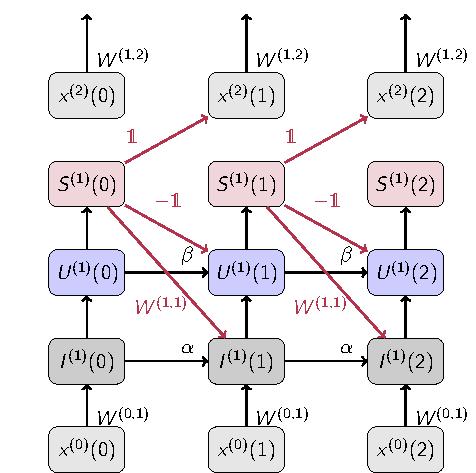
\includegraphics{figures/snn_graph.pdf}
	\caption{Illustration of the computational graph of a spiking neural network
  in discrete time. Time steps flow from left to right. Inputs $x^{(1)}$ are fed
	into the network from the bottom and propagate upwards to higher layers. The
	synaptic currents $I$ are decayed by $\alpha$ in each time step and feed
	into the membrane potentials $U$. The $U$ are similarly decaying over time
	as characterized by $\beta$. Spike trains $S$ are generated by applying a
	threshold nonlinearity to the membrane potentials $U$ in each time step.
	Spikes causally affect the network state (red connections).  First, each
	spikes causes the membrane potential of the neuron which emits the spike to
	be reset. Second, each spike may be communicated to the same neuronal
	population via recurrent connections $W^{(1,1)}$.  Finally, it may also be
	communicated downstream via $W^{(1,2)}$ to another downstream network layer
	or, alternatively, a readout layer on which a supervised cost function is
	defined.}
    \label{fig:snn_computational_graph}
\end{SCfigure}

Equations~\eqref{eq:syn_discrete_time} and~\eqref{eq:mem_discrete_time}
characterize the dynamics of a \gls{rnn}
(Figure~\ref{fig:snn_computational_graph}).  Specifically, the cell state of
neuron $i$ is characterized by the instantaneous synaptic currents $I_i$ and the
membrane voltage $U_i$.  
It is straightforward to evaluate these equations. Moreover, we can use
standard machine learning libraries with auto-differentiation capabilities to do so.
% TODO perhaps add a figure of a spiking neuron here (FRIEDEMANN)

% Segue to "training" and learning problem
We have how seen that \glspl{snn} constitute a special case of \glspl{rnn}.
However, so far we have not talked about how the weights in any \gls{rnn} should be set to implement a specific computational function.
Next we turn our attention to learning. 
In other words, we now focus on methods which permit us to systematically change the weights in a given network to implement a specific computational function.


\section{The \gls{rnn} learning problem (Hesham)}
Because \glspl{rnn} can be used in a variety of scenarios ranging from time series prediction, over language translation, to automatic speech recognition, powerful machine learning methods exist to train them. 
In the following we discuss the most common approaches before analyzing their applicability to \glspl{snn}.

The ingredients of the learning process are typically the same throughout.
The first ingredient is a cost function, or a loss, which is minimized when the network's response corresponds to the desired behavior.
In time series prediction for example, this loss could be the difference between the predicted and the true value.
The second ingredient is a mechanism that updates the network's weights so as to minimize the loss.
The simplest and yet powerful mechanism to achieve this is gradient descent.
It holds the solution to the spatial credit assignment.


\subsection{Spatial Credit Assignment (HM, EN, FZ)}
\label{sec:spatial_CA}

In multi-layer neural networks, gradient descent can be implemented efficiently using the backpropagation algorithm \refbox{box:bp}. 
In its simplest form, the backpropagation algorithm 
assigns credit (or blame) to the parameters, e.g.\ input weights of connected neurons, and computes how parameters should be updated differentially to yield an overall decrease in loss.
To achieve this, the algorithm propagates errors ``backwards'' from the output of the network to earlier upstream neurons.

Using backpropagation to adjust deep layer weights ensures that the weight update  will reduce the output layer error for the current training example (if the learning rate is small enough).
While this theoretical guarantee is highly desirable, it comes at the cost of more complex communication requirements, namely that errors have to be communicated back through the network, and increased memory requirements as the neuron states need to be buffered until the errors become available.
These requirements can be relaxed by either:
1)~Approximating the error backpropagation step through cheaper means that incur less memory, communication and computational overhead;
2)~Formulating an alternative learning problem where the errors for each neuron are proximally generated, both in space and time.
In the following, we describe examples of both type of solutions.

% TODO don't know what to do with this sentence
{\bf Description of non-locality and the problem with the non-differentiable spike generation non-linearity \refbox{box:nonlocal}}


\begin{infobox}
  \begin{mdframed}[backgroundcolor=black!10]\small
    \caption{\label{box:bp} The Gradient Backpropagation Rule} The task of learning is to minimize this cost over the entire dataset.
    This can be done efficiently using the gradient descent rule, which modifies the network parameters $\mathbf{w}$ in the direction opposite to the gradient:
    %
    \begin{equation}\label{eq:bp_shallow}
      \begin{split}
        w_{ij} \leftarrow w_{ij} - \eta \Delta w_{ij},  \text{where } \Delta w_{ij} = \frac{\mathrm{\partial}}{\mathrm{\partial} w_{ij}} L = \rho'\left(\sum_j w_{ij} x_j\right) e_i x_j,
      \end{split}
    \end{equation}
    %
    and where $\eta$ is a small learning rate. 
    In deep networks, the weights of the hidden layer neurons are modified by backpropagating the errors from the prediction layer using the chain rule. 
    Using superscripts $l=0,...,N$ to denote the layer ($0$ is input, $N$ is output):
    %
    \begin{equation}\label{eq:bp_deep}
      \frac{\mathrm{\partial}}{\mathrm{\partial} W^{l}_{ij}} L = \delta_{i}^{l}  S^{l}_j,\text{ where }\delta_{i}^{l} = \rho'\left( U_i^l \right) \sum_k \delta_{k}^{l+1}[t] W_{ki}^{l+1},
    \end{equation}
    where the $\delta_{i}^N=e_i$, as in Eq. \ref{eq:bp_shallow} and $y_{i}^0=x_i$.
    % 
    This update rule is ubiquitous in deep learning \cite{Rumelhart_etal88_paradist} and known as the gradient backpropagation algorithm.   
    Learning is typically carried out in forward passes (evaluation of the neural network activities) and backward passes (evaluation of $\delta$s).
  \end{mdframed}
\end{infobox}



\subsection{Temporal Credit Assignment (Emre)}
\label{sec:temporal_credit_assignment}

When training \glspl{rnn}, we do not only require a solution to the spatial credit assignment problem, but we also have to worry about temporal dimension of the network activity. Thus we also have to solve a temporal credit assignment problem.
Fortunately, both spatial and temporal credit assignment are related and we apply the same strategies by ``unrolling'' the network in time.
The recurrent neural network is ``unrolled'' meaning that an auxiliary network is created by making copies of the network for each time step (see Figure \ref{fig:snn_computational_graph}).
Applying backpropagation on such an ``unrolled'' network is referred to as \gls{bptt}.

When training \glsplw{rnn} the unrolled network can become ``deep'' quickly as the number of required timesteps is large. This temporal depth is accompanied with increased memory requirements which can quickly become prohibitive, especially when considering neuromorphic applications where memory is often scarce.

In some situations it can thus be beneficial to propagate all necessary information for gradient computation forward in time \cite{Williams_Zipser89_learalgo} (Fig. \ref{fig:backwrd_vs_forward_prop}).
%Some form of memory is required to solve the temporal credit assignment problem in \glspl{rnn}. 
In the following we briefly review the main differences between the two methods.
For illustration purposes here, we assume a neural network with $L$ layers and a cost function $\mathcal{L}[t] = \sum_i (U^{L}_i[t]-\hat{U^{L}_i}[t])^2$. 
%
\begin{figure}[htbp]
    \centering
    \subfloat[Backward Method]{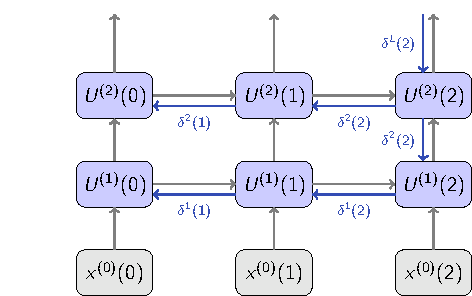
\includegraphics[width=.4\textwidth]{figures/diagram_bp}}
    \subfloat[Forward Method]{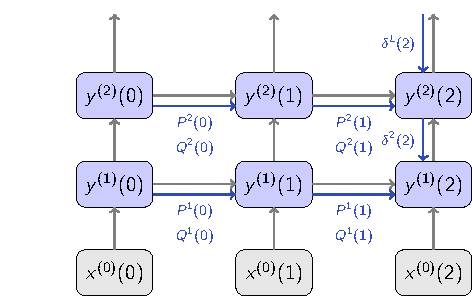
\includegraphics[width=.4\textwidth]{figures/diagram_rtrl}}
  \caption{\emph{Strategies for Temporal Credit Assignment}. (Left) At time $t=2$ Errors are propagated backwards. To compute the parameter updates, the states of every neuron ($U^{(i)}$, $I^{(i)}$, and $S^{(i)}$, $i=0,1,2$) and the inputs ($x^{(0)}$) for each time step are stored. (Right) At time t=2, all the information from previous time steps has been propagated forward. The nature of this information is determined by the network structure and neuron dynamics. Note that, in the forward method, the gradient step is backpropagated along the layers in time step $t=2$, but in isolation of the other timesteps. This backward step is challenging in itself, and solutions to achieve this in a local fashion are discussed in Sec.~\ref{sec:spatial_CA}. Nodes $y$ represent the nodes $S$, $U$, $I$ and $x$ for illustration purposes in this figure.
}. 
    \label{fig:backwrd_vs_forward_prop}
\end{figure}
%
\begin{enumerate}
\item The ``backward'' method:  
The unrolling of the network clarifies the flow of information in the inference and training stages (\reffig{fig:backwrd_vs_forward_prop}).
An important property of the unrolled network is that the parameters are shared across the time axis.
    Thus, the unrolled network is simply a deep network with shared weights on which one can apply the standard \Gls{bp} applies:
%
\begin{equation}\label{eq:bp_deep}
  \begin{split}
    \Delta {W_{ij}^{(l,l)}} &\propto \frac{\mathrm{\partial}}{\mathrm{\partial} W^{(l,l)}_{ij}} \mathcal{L}[T]  = \sum_{t=0}^T \delta_{i}^{l}[t]  S^{l-1}_j[t],\\
    \delta_{i}^{l} [t] & = \rho'\left( U_i^l [t] \right) \left( \sum_k \delta_{k}^{l+1}[t] W_{ki}^{(l,l+1)} + \sum_k \delta_{k}^{l}[t+1] W_{ki}^{(l,l)} \right),
  \end{split}
\end{equation}
%
where $T$ is the duration of the sequence, and using the notation $\delta^{L}_i[t] = U_i^L[t]-\hat{U}_i^L[t]$
This rule is known as \gls{bptt}, and the main difference compared to \gls{bp} is the sum over time steps $t$.
\gls{bptt} solves the temporal credit assignment problem by back propagating through the unrolled network.
This method works backward through time after completing a forward update.
In practice this is an expensive operation, as the entire history of activation must be buffered to computed the gradients.
The use of standard backpropagation on the unrolled network directly enables the use of autodifferentiation tools offered in model machine learning toolkits~\cite{Bellec_etal18_longshor,Shrestha_Orchard18_slayspik,Wozniak_etal18_deepnetw}.\\
\item The forward method: The information required for computing the errors is propagated forward.
%Use Williams and Zipser equations, and explain special case where the ODE has a solution = superspike
  For a \gls{lif} neuron with first order dynamics, recall that the discrete-time membrane potential and synaptic current can be expressed as Eqs.~\eqref{eq:syn_discrete_time} and \eqref{eq:mem_discrete_time}.
%\[
%\begin{split}
%U_i[t+1] & = \beta U_i[t] + I_i[t]\\
%  I_i[t+1] & = \alpha I_i[t] + \sum_j W_{ij} \sigma(U_j[t])
%\end{split}
%\]
The gradient of a cost function $\mathcal{L}[t]$ with respect to weight $W_{ij}$ is then:
\[
\begin{split} \label{eq:forward_mode_differentiation}
 \Delta {W_{ij}} &\propto \frac{\partial }{\partial W_{ij}} \mathcal{L}[t+1] = \delta_i[t+1] P_{ij}[t+1]\\
 P_{ij}[t+1]     &= \frac{\partial} {\partial W_{ij}}  U_i[t+1] = \beta P_{ij}[t] + Q_{ij}[t] + \sum_j W_{ij} \sigma'(U_j[t-1]) P_{ij}[t-1]\\
 Q_{ij}[t+1]     &= \frac{\partial} {\partial W_{ij}}  I_i[t+1] = \alpha Q_{ij}[t] + \sigma(U_i[t]) + \sum_j W_{ij} \sigma'(U_j[t-1]) P_{ij}[t-1],
\end{split}
\]
Here, we replaced the spiking variable $S_j$ with the smooth activation function $\sigma(U_j[t])$.

where $\sigma'$ is the derivative of $\sigma$.
\end{enumerate}


%Asymptotic Complexity Analysisconclusion(incomplete)
In conclusion, both solutions transform the temporal credit assignment problem to a spatial one and then apply the same strategy as for spatial credit assignment (cf.\ \refsec{sec:spatial_CA}).
The backward approach is more efficient in terms of computation, but requires maintaining all the inputs and activations for each time step.
Thus the space complexity of the backward approach is $O(N T)$, where $N$ is the number of neurons.\\
On the other hand, the forward method requires maintaining variables $P_{ij}$ and $Q_{ij}$.
The space complexity is $O(N^2)$, where $N$ is the number of neurons.
In a single layer feed-forward architecture without refractory mechanisms, the third term above vanishes and $P_{ij}$, $Q_{ij}$ no longer depend on $j$.
In this case, the space complexity becomes $O(N)$.
This simplification can lead to an efficient synaptic plasticity rule for deep local learning, as described later.

As memory is ample in modern von Neumann computers, the backward method is preferred for an implementation on a conventional computer.
On the other hand, processing in dedicated neuromorphic hardware and, more generally, non-von Neumann computers may not have immediate access to such large memory.
In this case, the forward approach is preferable.
Furthermore, the forward approach is appealing from a biological point of view, since the learning rule is consistent with synaptic plasticity in the brain and ``three-factor'' rules.

%%Error-triggered learning
%Learning on a non-local substrate means that the weight updates must be performed in a non-local fashion as well.
%Importantly, if training is performed epochwise (meaning weights are updated at the end of a sequence), a separate memory is required to accumulate the incremental weight updates.
%In the equation \ref{eq:integral_superspike}, this memory is implicitly assumed by the integral.
%Alternatively, the weights can be updated incrementally, meaning a weight update is performed at every time step, or when the instantaneous local error exceeds a threshold as in 
%\textbf{Challenge: continuous dynamics= continuous weight change. Solution: Error-triggered learning} \cite{Neftci18_datapowe}.




% Segue to spiking neuron case to describe problem of non-differability
In summary, efficient algorithms exist to train train \glspl{rnn}.
An important requirement for these algorithms to work, however, is that the involved networks are differentiable.
Differentiability is one of the core difficulties we have to overcome to train a \gls{snn}.
We will discuss the main challenges to successfully train \glspl{snn} in the following. 


\subsection{Challenges for credit assignment with spiking neurons}

Like in the case of \glspl{rnn}, training \glspl{snn} requires to efficiently solve spatial and temporal credit assignemnt. 
Before the algorithms introduced above can be applied to \glspl{snn}, and to neuromorphic hardware specifically, two two key challenges need to be overcome.

The first challenge, concerns the lack of differentiability of the spiking nonlinearity itself. 
We can appreciated this fact by inspection of Equations~\eqref{eq:bp_deep} and~\eqref{eq:forward_mode_differentiation}.
Both expressions contain the partial derivative $\rho^\prime$ of the activation function $\rho$ as a multiplicative factor.
For our spiking neuron, however, we have $\rho(U(t))=S(U(t))=\Theta(U(t)-\vartheta)$ (cf.\ Eq.~\eqref{eq:spike}) and thus 
\begin{equation}
\rho^\prime(U(t))=\frac{\partial \rho(U(t))}{\partial U(t)}=
\begin{cases}
0 & U\ne\vartheta\\
\infty & U=\vartheta
\end{cases}
\end{equation}
Thus the gradients evaluate to either~$0$ or~$\infty$ respectively which makes them unsuitable for gradient based optimization.
In summary, the ``hard'' all-or-nothing character of the binary spiking nonlinearity stops gradients from ``flowing'' whenever error signals are to be propagated.
It is worth noting, that the same issue occurs in binary neural networks and some of the proposed solutions described below were first introduced in binary networks . 
% TODO CITE bengio straight through paper and hinton coursera lecture

The second challenge, mostly concerns the memory requirements of temporal and layer-wise error propagation.
% TODO formulate precisely what the second problem is here 
---missing paragraph---


\section{Solutions to the credit assignment problem with spiking neurons}
To overcome the challenge of the ``hard'' spiking nonlinearity limitation, several approaches have been devised to train \glspl{snn} with varying degrees of success. The most common approaches can be coarsely classified into the following categories: 
  i)~resorting to entirely unsupervised learning for the hidden units, 
 ii)~translating conventionally trained ``rate-based'' neural networks to spiking neural networks,
iii)~smoothing the network model to be continuously differentiable, or 
 iv)~defining a surrogate gradient as a continuous relaxation of the real
gradients.  
Approaches pertaining to unsupervised learning and network translation have been reviewed extensively in \cite{tavanaei_deep_2018}. 
In this tutorial we focus on the latter two supervised approaches which we will refer to in the following as the ``smoothed'' and \gls{sg} approach.
%% Move following to body
%The main difference between the two is that smoothed approaches entail modifications to the forward pass of the network dynamics by either dispensing with binary nonlinearities, by using specific coding schemes, or by introducing stochasticity.  
%\Gls{sg} methods on the other hand leave the forward pass unchanged and act solely on the learning dynamics. 
We will first briefly review existing literature on common ``smoothing'' and \gls{sg} approaches before turning to an in-depth discussion of how to build functional spiking neural networks. 


\section{Smoothed spiking neural networks (Friedemann)}

% Truly smooth models (smooth forward pass)
The defining characteristic of smoothed \glspl{snn} is that their formulation ensures well-behaved gradients which are directly suitable for optimization.
Smooth models can be further categorized into soft nonlinearity models, probabilistic models, for which gradients technically are only well defined, or models which either rely on rate-codes or
single-spike temporal codes.  


\subsection{Gradients in soft nonlinearity models}

This approach can in principle be applied
directly to all spiking neuron models which explicitly include a smooth spike
generating process. This includes, for instance,  the Hodgkin-Huxley,
Morris-Lecar, and FitzHugh-Nagumo models \cite{Gerstner_etal14_neurdyna}.
However, in practice this approach has only been applied successfully by
\cite{Huh_Sejnowski17_graddesc} using an augmented integrate-and-fire model in
which the binary spiking nonlinearity was replaced by an continuous-valued
gating function.  The resulting network constitutes a \gls{rnn} which can be
optimized using standard methods of \gls{bptt} or \gls{rtrl}.  

% Discussion of shortcomings
It remains unclear, however, how spike reset dynamics should be coupled into
such models. More importantly, the soft threshold models compromise on one of
the key features of \gls{snn}, namely the binary activation function which is
essential for power efficiency.


% Probabilistic models (probabilistic forward pass)
\subsection{Gradients in probabilistic models}

Another example for smooth models are binary probabilistic models. 
Binary probabilistic models have been objects of extensive study in the machine
learning literature mainly in the context of (restricted) Boltzmann machines
for which efficient local learning rules exist \cite{ackley_learning_1985}. 
Similarly, the propagation of gradients has been studied for binary stochastic
models \cite{bengio_estimating_2013}. 
In simple terms, stochasticity effectively smooths out the hard binary
nonlinearity which makes it possible to define a gradient on expectation values.
\glspl{sg} approaches, as we will elucidate below, are direct extensions of
these ideas to the class of more domain specific spiking neuron models without
the need for stochasticity.  
% TODO this needs some more careful research ... 

% Learning in probabilistic spiking framework
In the neurosciences, the utility of probabilistic models 
has first been appreciated because it allows to formally define the smooth
log-likelihood of a spike train which can be optimized using gradient descent
\cite{pfister_optimal_2006}.
Although this insight was first discovered in networks without hidden units,
the same ideas were later extended to multi-layer networks with a single hidden
layer \cite{gardner_learning_2015}.
% Both add hidden units (variational learning approach)
In a similar vein, variational learning approaches have been proven capable
in learning useful hidden layer representations in \glspl{snn}
\cite{brea_matching_2013, rezende_stochastic_2014,Mostafa_Cauwenberghs18}.
However, at the same time the injected noise necessary to smooth out the effect
of binary nonlinearities has proven challenging to optimize
\cite{rezende_stochastic_2014}.


% f-I curve based approaches
\subsection{Gradients for rate-based codes}

Another common approach to obtain gradients in spiking neural networks is to
assume a rate-based coding scheme.
The main idea is that spike rate is the underlying information-carrying quantity.
For many plausible neuron models, the supra-threshold firing rate depends
smoothly on the neuron input. This input-output dependence is captured by the
so-called f-I curve of a neuron.
In such cases, the derivative of the f-I curves is suitable for gradient-based optimization. 

% TODO add figure to distinguish between rate and spike coding

There are several examples of this approach. 
For instance \citet{Hunsberger_Eliasmith15_spikdeep} used an effectively
rate-coded input scheme to demonstrate competitive performance on standard
machine learning benchmarks such as CIFAR10 and MNIST.
A similarly \cite{Lee_etal16_traideep} demonstrated deep learning in spiking
neural networks using ... % TODO is this translation ?

% Discussion of pros & cons
Rate-based approaches can offer good performance, but they may be inefficient.
On the one hand, precise estimation of firing rates requires averaging over
a number of spikes.  Such averaging requires either relatively high firing rates or
time because several repeats are needed to average out discretization noise.  
To some degree this problem can be overcome by spatial averaging over
large populations of spiking neurons. However, this may comes at the expense of
more neurons. 
Alternatively, temporal and resource limitations could be overcome by instead relying on
spike timing as the information-carrying quantity. This is the idea behind
spike timing based coding.


% Single spike time codes
\subsection{Gradients for single spike timing based codes}

In an effort to optimize \glspl{snn} without potentially harmful noise
injection and without reverting to a fully rate-based coding scheme, 
several studies have formulated spiking neural
networks as a set of firing times.
In such a temporal coding setting, individual spikes can carry significantly more
information compared to rate-based schemes.

When using a purely firing time based code, the information carrying quantity is
firing time which can depend smoothly on neuronal inputs as long as a hidden
unit does not fall quiescent.
The idea of single spike temporal coding was 
pioneered in SpikeProp \cite{bohte_error-backpropagation_2002}.
In this work the analytic expressions of firing times for hidden units 
were linearized, allowing to compute approximate hidden layer gradients fully
analytically. 
Several variations and extensions of this approach have been developed,
to cope with, for instance, multiple hidden layers and spikes
\cite{banerjee_learning_2016}. % TODO needs work here
More recently, a similar approach without the need for linearization 
was used in \cite{Mostafa16_supelear} where the author computed the spike timing 
gradients explicitly for non-leaky integrate-and-fire neurons. 
Intriguingly the work, showed to yield competitive performance to conventional
networks on MNIST.
% TODO Should write a little more, @Hesham would the right person to write this
% and also to check whether this is correct

% Discussion & Limitations
Although the spike timing formulation does in certain cases
yield well-defined gradients, it may suffer from certain
limitations. 
For instance, the formulation of SpikeProp required each hidden
unit to emit exactly one spike per trial. Moreover, it is difficult to define 
firing time for quiescent units, although population sparseness, as it is
ubiquitously found in the brain, is presumably crucial for power
efficiency.
% TODO @Hesham ?


\section{Surrogate gradients (Friedemann)}
\label{sec:surrogate_gradients}

To overcome some of the difficulties which are associated with training \glspl{snn}, we now introduce the notion of \gls{sg} methods.
Their defining characteristic is that instead of changing the model definition, a \gls{sg} is introduced as a continuous relaxation of the non-smooth spiking threshold for purposes of numerical optimization.
Importantly, this approximation is only used in the parameter updates and does not affect the forward pass of the network directly.
The use of \glspl{sg} allows to efficiently train \glspl{snn} without specifying whether a temporal or spike-timing based coding scheme is to be used. 

Like vanilla gradient-descent, \gls{sg} learning can deal with the spatial and temporal credit assignment problem by either \gls{bptt}, by forward-propagation of all relevant information through eligibility traces (see Section~\ref{sec:temporal_credit_assignment} for details), or, alternatively, by introducing additional approximations which can offer advantages specifically for hardware implementations. 
% We are still missing the notion of local and global, fzen
In the following we briefly review existing work relying on \gls{sg} methods before turning to a more in-depth treatment of the underlying principles and capabilities. 


\subsection{Surrogate partial derivatives for spiking nonlinearity}
A set of works have used \gls{sg} to specifically overcome the challenge of the ``hard'' nonlinearity. 
In this works typically a standard algorithm such as \gls{bptt} is used with on minor modification: within the algorithm each occurrence of the partial derivative of the spiking nonlinearity is replaced by the derivative of a smooth function.
Implementing these approaches is possible in most auto-differentiation-enabled machine learning libraries by minor extensions (e.g.\ Tensorflow and PyTorch).
Because all other aspects of backpropagation remain unaffected, these algorithms typically do not change the non-locality of the update rules. 

One of the first uses of such a \gls{sg} is described in
\citet{bohte_error-backpropagation_2011} where the partial derivative of a
spiking neuron was approximated by the derivative of a \gls{relu}.
This is similar in flavor to the solution proposed in 
\citep{courbariaux_binarized_2016} to optimize binary neural networks. 
Essentially the same idea underlies the training of large-scale
convolutional networks with binary activations on classification problems using neuromorphic hardware \cite{esser_convolutional_2016}.
However, here the authors used a modified \gls{relu} as the surrogate partial derivative.
Recently, \cite{Bellec_etal18_longshor} successfully trained networks of 
neurons with slow temporal dynamics using the same surrogate derivative. 
Encouragingly, the  authors found that such networks can perform at par with conventional \gls{lstm} networks.
Similarly, \citet{Wozniak_etal18_deepnetw} reported competitive performance on a series of temporal benchmark datasets.
\citet{Shrestha_Orchard18_slayspik} used a an exponential function and reported competivie performance on a range of neuromorphic benchmark problems.



% TODO need to sort the papers below into above categories
% \cite{OConnor_Welling16_deepspik} % TODO Not sure I understand this paper and whether this qualifies as SG need to. Emre: I think we can omit this. Emre: Let's omit for the time being. Fzen: LOL

% TODO need to add https://arxiv.org/abs/1812.07040
% TODO need to add Slayer paper 

% Spiking Expectation Maximization \cite{Nessler_etal13_bayecomp}, 
% temporal codes for deep learning with spikes \cite{OConnor_Welling16_deepspik}, 
% train-and-transfer techniques \cite{Esser_etal16_convnetw}, 
% and predictive coding \cite{Deneve_etal17_braieffi}.



\subsection{Surrogate gradients affecting locality of the update rules}

The algorithms discussed in the last section only constitute a minor modification of \gls{bptt}. As such, their memory requirements can be substantial, especially when long time sequences are to be processed in the network.
In the following we discuss \gls{sg} approaches which introduce far larger deviations from the true gradients which allow for learning often at a greatly reduced computational cost or implementational complexity.



\begin{figure}
  \centering
  \subfloat[BP]{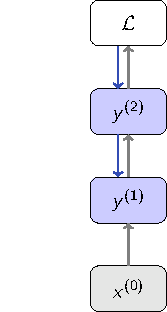
\includegraphics[height=10em]{figures/spatial_ca_bp.pdf}}
  \subfloat[Feedback Alignment]{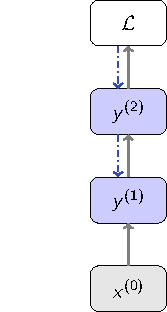
\includegraphics[height=10em]{figures/spatial_ca_fa.pdf}}
  \subfloat[Random BP]{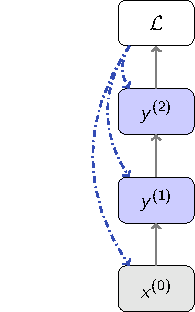
\includegraphics[height=10em]{figures/spatial_ca_rbp.pdf}}
  \subfloat[Local Errors]{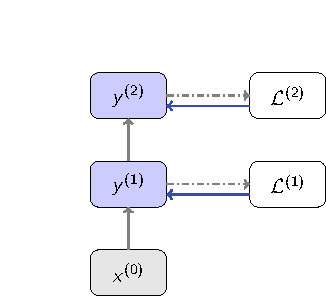
\includegraphics[height=10em]{figures/spatial_ca_dll.pdf}}
  \caption{\emph{Spatial error credit assignment and strategies for relaxing gradient \Gls{bp} requirements}. Dashed lines indicate random connections}
\end{figure}


\subsubsection{Random Error \Gls{bp}}
One family of algorithms that relaxes the symmetry requirement of \Gls{bp} are feedback alignment or random \Gls{bp} algorithms \cite{Lillicrap_etal16_randsyna,Baldi_etal16_learmach}. 
These are approximations to the gradient \Gls{bp} rule that side-step the non-locality problem by replacing weights in the learning channel with random ones, leading to remarkably little loss in classification performance on benchmark tasks (requirement (i) in \refbox{box:bp}). 
Although a general theoretical understanding of random \Gls{bp} is still a subject of intense research, extended simulations of linear networks show that, during learning, the network adjusts its feed-forward weights such that they align with the (random) feedback weights, which are effective in communicating gradients \cite{Lillicrap_etal16_randsyna}.
Building on these findings, an asynchronous spike-driven adaptation of random \Gls{bp} using local synaptic plasticity rules with the dynamics of spiking neurons was demonstrated \cite{Neftci_etal17_evenrand}.
%The \ac{eRBP} rule was tested on software simulations of digital neuromorphic hardware \cite{Detorakis_etal17_neursyna}, with fixed width representations for neural states and synaptic weights \reffig{fig:erbp}.
Extended experimentations with \Gls{eRBP} show that the spiking nature of neuromorphic hardware and the lack of complex non-linear computations at the neuron do not prevent accurate learning on classification tasks, and can operate continuously and asynchronously without alternation of forward or backward passes.
Up to moderate classification accuracies, a spiking implementation requires an equal or fewer number of synaptic operations (SynOp) compared to multiply accumulation (MAC) operation to reach a given accuracy for both networks \cite{Neftci_etal17_evenrand}.
While a standard computer remains the architecture of choice if classification accuracy on a stationary dataset is the target regardless of energy efficiency, neuromorphic hardware is a strong contender if low-power learning on non-stationary data is the objective, since energy efficiency is improved at least by a factor equal to the achieved Joule/MAC to Joule/SynOp ratio and learning is on-going.


\subsubsection{Learning Using Local Errors} 
Multi-layer neural networks are hierarchical feature extractors.
Through successive linear projections and point-wise non-linearities, neurons become tuned (respond most strongly) to particular spatio-temporal features in the input.
While the best features are those that take into account the subsequent processing stages and which are learned to minimize the final error(as the features learned using backpropagation do), high-quality features can also be obtained by more local methods.
The non-local component of the weight update equation (Eq.~\ref{eq:bp_deep}) is the error term $\delta_i^l[t]$.
Instead of obtaining this error term through backpropagation, we require that it be generated using information local to the layer. 
One way of achieving this is to define a layer-wise loss $E^l({\bf y}^l[t])$ and use this local loss to obtain the errors.
In such a local learning setting, the weight update equation becomes:
%
\begin{equation}\label{eq:bp_local}
  \frac{\mathrm{\partial}}{\mathrm{\partial} W^{(l-1,l)}_{ij}} \mathcal{L}^l = -\sum_{t=0}^T \delta_{i}^{l}[t]  y^{l-1}_j[t],
    \text{ where }
    \delta_{i}^{l} [t] = \rho'\left(\sum_j W^{(l-1,l)}_{ij} y^{l-1}_j [t] \right) \frac{\mathrm{d}}{\mathrm{d}y_i^l[t]}\mathcal{L}^l({\bf y}^l[t])
\end{equation}
One convenient form for the local loss that works well in practice is:
\begin{equation}
\mathcal{L}^l({\bf y}^l[t]) \equiv \mathcal{L}({\bf W}^l_{r} {\bf y}^l[t],\hat{{\bf y}}^{l}[t])
\end{equation}
%
where $\hat{{\bf y}}^{l}[t]$ is a pseudo-target for layer $l$, ${\bf W}_l^{r}$ is a fixed random matrix that projects the activity vector at layer $l$ to a vector having the same dimension as the pseudo-target, and $\mathcal{L}$ is a function measuring the discrepancy between its two arguments.
In essence, this formulation assumes an auxiliary random layer is attached to layer $l$ and the goal is to modify ${\bf W}^{(l-1,l)}$ so as to minimize the discrepancy between the auxiliary random layer's output and the pseudo-target. 
The simplest choice for the pseudo-target is to use the top-layer target. 
This forces each layer to learn a set of features that are able to match the top-layer target after undergoing a fixed random linear projection. Each layer builds on the features learned by the layer below it, and we empirically observe that higher layers are able to learn higher-quality features that allow their random and fixed auxiliary layers to better match the target.
\label{sec:spatial_credit_assignment}


\begin{infobox}
  \begin{mdframed}[backgroundcolor=black!10]\small
    \caption{\label{box:nonlocal} Non-local Models of Computation}
     Locality of computations is characterized by the set variables available to the physical processing elements, and depends on the computational substrate.
    Information necessary for learning can be non-local (it is available elsewhere), or global (it is shared among all processing elements).\\
    To illustrate the concept of locality, we assume two neurons, $A$ and $B$, and would like Neuron $A$ to implement a function on domain $D$ defined as:
    \[ 
      \begin{split}
        D & = D_{loc} \cup D_{nloc},\\
        \text{where } &D_{loc}=\{w_{BA},S^A(t), u_A(t)\}\text{ and }D_{nloc} = \{ S^B(t-T), u_{B}\}.
      \end{split}
    \]
    Here, $S^B(t-T)$ refers to the output of neuron $B$ $T$ seconds ago, $U_A$, $U_B$ are the respective membrane potentials, and $w_{BA}$ is the synaptic weight from $B$ to $A$.  
    Variables under $D_{loc}$ are directly available to Neuron A and are thus local to it. 
      
    On the other hand, variable $S^B(t-T)$ is temporally non-local and $u_{B}$ is spatially non-local to neuron $A$.
    Spatially global signals are often required for learning on practical tasks, and even commonplace in the brain (\emph{e.g.} neuromodulation).
    Non-local information can be transmitted through special structures, for example dedicated encoders and decoders for $U_B$ and a form of working memory for $S^B(t-T)$.
    An important challenge is to map relevant computations on functions of $D$ by minimizing the cost of communicating $D_{nloc}$.
    
  \end{mdframed}
\end{infobox}


\subsubsection{SuperSpike} 
% TODO write a section on SuperSpike
% biologically plausible
Finally, \citet{zenke_superspike:_2018} using yet another surrogate derivative in combination with a forward propagation to derive an biologically plausible online
learning rule to learn precisely timed spike train transformations. 




% END OF THIS SECTION


\section{NEEDS MOVING Credit Assignment in Spiking Neural Networks}
\label{sec:credit_assignment}
% Not sure where to move this section to, fzen

% \begin{comment}
% Ideas for credit assignment classification:
% 
% (Figure: step-function sigmoid)
% 
% * temporal credit assignment
%     *    back-prop-like, e.g. Bellec et al., SLAYER (Figure: flow of error information in time -- with the next point)
%     *    forward in time (single hop), e.g. SuperSpike
%     *    ignored, don't talk about it (I think most rate-based approaches, because essentially assume a temporal steady state)
%     
% * spatial credit assignment
%     * back-prop-like
%     * random feedback (direct feedback, feedback alignment, etc)
%     * local error learning
% \end{comment}


In gradient-based learning, the parameter updates contain a term that relates to the local error or, more generally, the derivative of the loss.
In a neural network, this term is affected by the computations downstream from the node containing the trained parameter.
This relationship is caused by the necessity to assign credit to that node, but its target value is not provided.
In conventional neural networks, this \emph{credit assignment problem} is solved by backpropagating the errors from the output layer using the chain rule (\emph{i.e.} the gradient BP rule).
The gradient BP rule relies on the immediate availability of backpropagated errors represented with high-precision memory.
In conventional computers, \Gls{bp} requires storage that is shared across connected nodes in the graph.
This type of shared memory does not exist in the brain, as states and parameters are local to the neurons and synapses \refbox{box:nonlocal}.
%In other words, to solve the credit assignment problem, errors need to be available at the right place and the right time. 
Non-locality can be spatial or temporal, or both.
To solve spatial non-locality, a special communication channel that transmits the errors to the relevant nodes must be provisioned \cite{Baldi_Sadowski16_theoloca}. 
To solve temporal non-locality, some form of (working) memory is required to maintain the history of the relevant states. 
Non-localities, both temporal and spatial, are arguably the most challenging and constraining aspect of spiking neural networks and synaptic plasticity \cite{Neftci18_datapowe}. 
Although non-locality in a model of computation can be seen as a serious shortcoming, it enables a tremendous advantage compared to conventional computer: massively parallel computing with carefully controlled (and potentially dynamic) interprocess communication. 
Thus, solving the ability to learn and process using local information extends well beyond the neuroscientists' agenda: it can enable information processing systems that approach the reliability and energy-efficiency of the brain.
In the following two sections, we describe solutions to the spatial and temporal credit assignment problems in spiking neural networks.



\section{Implementation}

\section{Application: Learning Gesture Recognition}
We demonstrate that deep learning algorithms that locally approximate the gradient backpropagation updates using locally synthesized gradients enable synaptic plasticity in spiking neural networks \cite{Kaiser_etal18_synaplas}.
This approach uses the forward method to overcome temporal credit assignment and local errors to overcome spatial credit assignment. 
To enable an efficient implementation in GPUs, the neuron model is simplified by omitting recurrent weights, including refractory mechanisms, in the backward pass. This omission results in a forward method that scales as $O(N)$ (instead of $O(N^2)$ for the full forward method).
\begin{equation}
  \text{Equations here or not?}
\end{equation}
The result is a highly efficient synaptic plasticity rule for multi-layer spiking neural networks.
Furthermore, our method utilizes existing autodifferentation methods in machine learning frameworks to systematically derive synaptic plasticity rules from task-relevant cost functions and neural dynamics. 
We benchmark our approach on the DVS Gestures dataset \reffig{fig:dcll_gestures}. 
\begin{figure}
  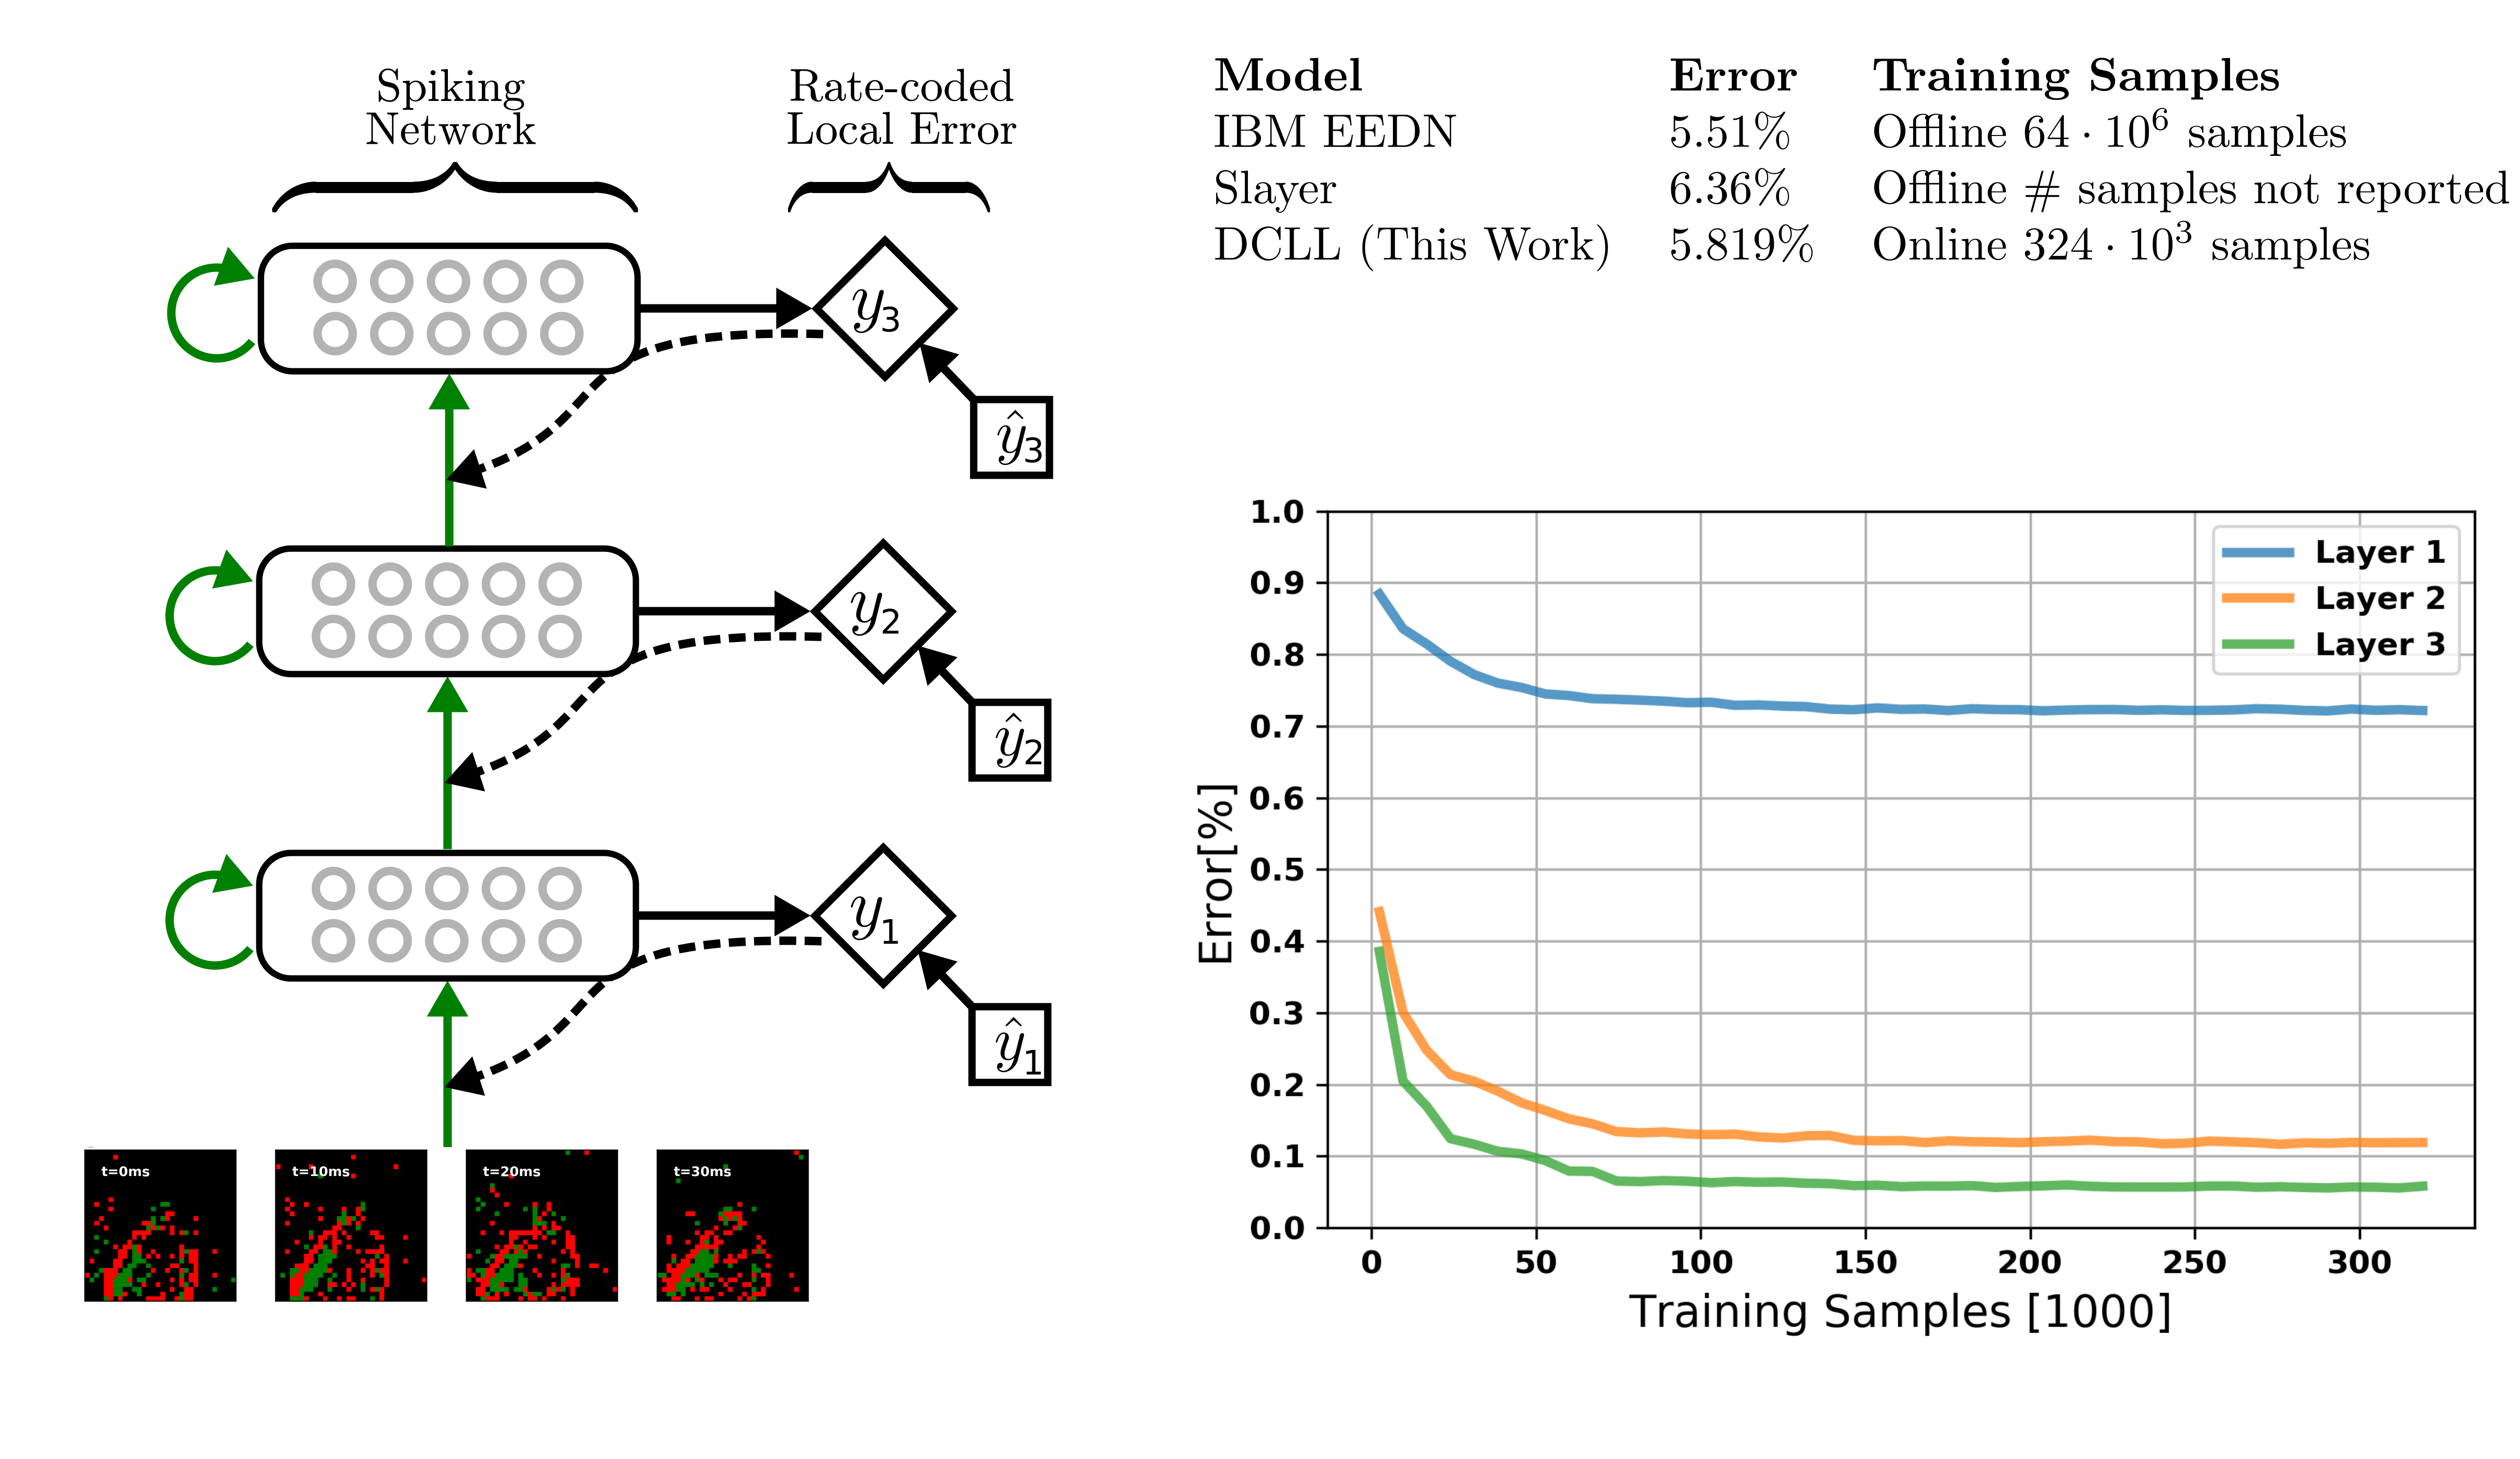
\includegraphics[width=.9\textwidth]{figures/DCLL_illustration.pdf}
  \caption{\label{fig:dcll_gestures} Deep Continuous Local Learning (DCLL) with spikes, applied to the DVSGestures dataset \cite{Amir_etal17_lowpowe}. A three layer convolutional spiking neural network is trained with \gls{sg} using local errors generated using fixed random projections to a local classifier. Learning in DCLL scales linearly with the number of neurons thanks to local rate-based cost functions formed by spike-based basis functions. Thanks to the \gls{sg} approach, the plasticity dynamics (dashed line) are synthesized with automatic differentiation under pyTorch. Results here are shown for the DVS Gestures dataset, 11 gestures recorded using a Dynamic Vision Sensor.}
\end{figure}

\section{Discussion}



%\section{Outline}
%%%%%%%% 
%\subsection{Introduction}
%This section covers the key characteristics of biological neural networks  \cite{Gerstner_Kistler02_spikneur}, including their dynamics, their potential for robust coding and efficient communication, and the consequences of computing on a physical substrate. 
%Next, it categorizes existing approaches to train \glspl{snn}, contrasting bottom-up and top-down (normative) theories, temporal vs. rate-based ones, and the capabilities of the state-of-the-art in each category. It will discuss the computational features of \glspl{snn} compared to artificial neural networks, their implementation in hardware, and the promises of \glspl{snn} to advance mobile, automotive and medical technologies.
%
%\subsection{Learning in Computational Neuroscience} 
%{\color{red} Merge with intro section.\\ }
%This section describes formally the traditional learning dynamics used in computational neuroscience, such as Hebbian learning in Hopfield networks, \glspl{stdp} \cite{masquelier_unsupervised_2007, tavanaei_deep_2018}, and reservoir models \cite{Buonomano_Maass09_statcomp,Sussillo_Abbott09_genecohe,Huang_etal06_extrlear}. 
%Following from the categorization in the introduction, this section covers classic gradient-based learning without hidden units, such as learning precisely timed output spike trains \cite{memmesheimer_learning_2014}, ReSuMe \cite{ponulak_supervised_2009}, the Tempotron \cite{Gutig_Sompolinsky06_tempneur}, the Chronotron \cite{florian_chronotron:_2012}. 
%The section continues describing prior approaches to learning with hidden units\cite{gardner_learning_2015}, including SpikeProp \cite{bohte_error-backpropagation_2002}, NormAD \cite{Kulkarni_etal17_learreal}, Spiking Expectation Maximization \cite{Nessler_etal13_bayecomp}, temporal codes for deep learning with spikes \cite{OConnor_Welling16_deepspik}, train-and-transfer techniques \cite{Esser_etal16_convnetw}, and predictive coding \cite{Deneve_etal17_braieffi}.
%% A common limitation in these methods is their inability to solve credit assignment in both temporal and spatial domains in deep networks. Consequently, there is space for improvement for efficient and accurate data-driven learning in \glspl{snn}.
%
%\begin{figure*}
%\centering 
%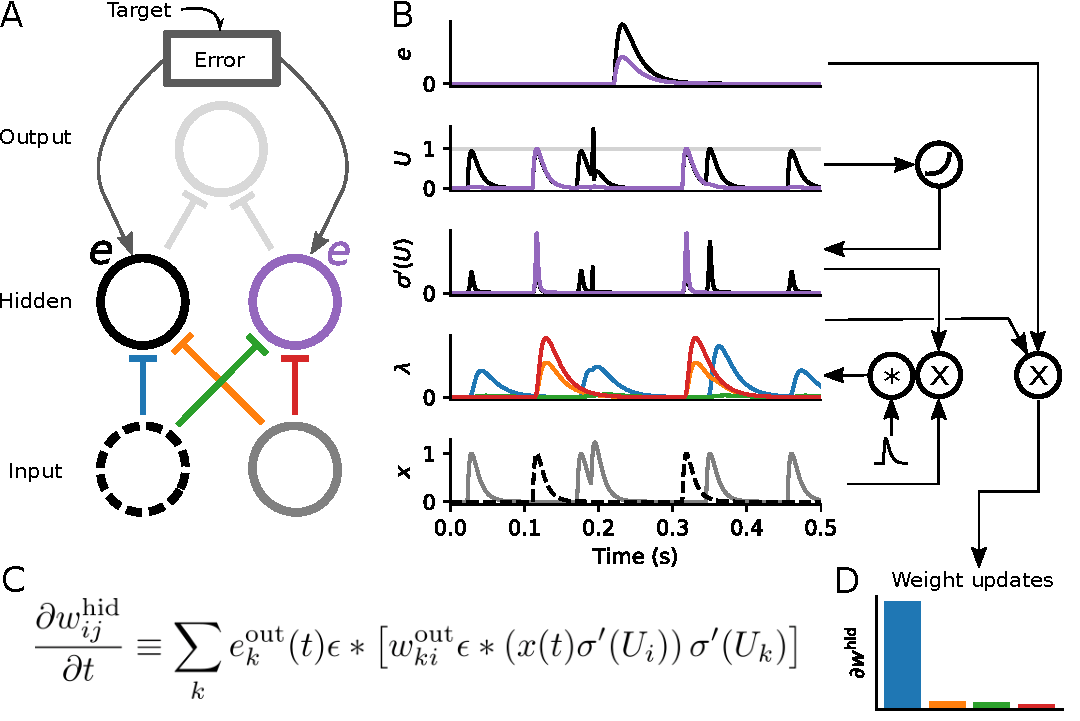
\includegraphics[width=3.0in]{./figures/superspike_concept.pdf}
%\caption{Example of SuperSpike learning of precisely timed target spikes in a three layer network.
%\textbf{A} Illustration of the network layout. Error signals are computed at the top using the van Rossum distance to the target spike train. These error signals are then send to the output unit and the hidden layer units. 
%\textbf{B} Time series of relevant quantities during one learning step. From top to bottom: $e$: The error signals as received by the two hidden units. $U$: The membrane voltage of the hidden units. $\sigma^\prime(U)$: The surrogate gradient for the hidden-layer spike trains ($S(U)$) which is computed from $U$ by applying a suitable monotonic nonlinearity which peaks at the firing threshold. $\lambda$: The four eligibility traces of the four hidden layer synapses. The eligibility traces are obtained by multiplying $x$ and $\sigma^\prime$ and further filtering them with the kernel of the van Rossum distance. $x$: The filtered input spike trains.
%\textbf{C} Weight update rule with symmetric feedback weights and without straight through estimation of downstream activities.
%\textbf{D} Bar chart of the weight updates in this example. The final weight updates are obtained by computing the product of the local error signals $e$ with the corresponding eligibility traces. In this example, increasing the blue synapse would be most beneficial for the network to minimize the output error.
%\label{fig:superspike_concepts}}
%\end{figure*}
%
%\subsection{Gradient-based Learning in \glspl{snn}} 
%This section describes a different type of gradient-based learning that is gaining significant momentum for training deep \glspl{snn} on practical tasks.
%It starts by describing the theory of gradient-based learning in multilayer artificial and biological neural networks \cite{Neftci18_datapowe}, using layman mathematical formulas. It follows with a mathematical description of spike-based computing and its relationship with binary neural networks. In the light of the provided mathematical formulas, the section underlines the physical nature of neural computation, and that, through the concept of the learning channel \cite{Baldi_etal17_learmach},  locality in learning equates with efficiency. Next, the section describes continuous relaxations of \glspl{snn}, namely the \glspl{sg} descent approach (see motivation).
%An overview of important prior work \cite{Esser_etal16_convnetw, courbariaux_binarized_2016, bellec_long_2018} will be following by the authors' related work on this topic, namely Random Backpropagation \cite{Neftci_etal17_evenrand}, Deep local learning \cite{Mostafa_etal17_deepsupe}, their extension to spiking networks using deep continuous local learning (Fig.~\ref{fig:dcll}), and SuperSpike 
%(Fig.~\ref{fig:superspike_concepts}; \cite{zenke_superspike:_2018}).
%Formally, this section concludes by underlining the bridges \glspl{sg} learning offers with the rich literature of machine learning and deep learning, and how this can lead to practical solutions, for example in reinforcement learning.
%
%\subsection{Approaches and tools for simulations and emulations of \glspl{snn}}
%{\color{red} Describe PyTorch and/or Auryn sims here\\ }
%An important obstacle in \glspl{snn} research is the prescription and simulation of large networks capable of solving problems routinely tackled in deep neural networks. This section argues that \gls{sg} learning in SNNs greatly facilitates this endeavor, as it naturally lends itself to the automatic differentiation tools \cite{Neftci18_datapowe} of machine learning frameworks. The section concludes by providing step-by-step instructions for running large-scale (up to 1M neurons) simulations of \glspl{snn} with \gls{sg} learning in pyTorch.
%
%\subsection{Applications and Benchmarks of \glspl{snn}}
%{\color{red} Gear this for signal processing\\ }
%\glspl{snn} can be viewed as a subclass of recurrent artificial neural networks. As such, they are best applied to problems dealing with dynamical environments, and in tasks where privacy and energy are paramount. This section will provide a table of benchmark datasets that are well suited to \glspl{snn}. Furthermore, we will provide a detailed example in DVS sensor data processing (Fig.~{fig:dcll}).
%
%\subsection{Conclusion}
%A brief conclusion summarizing the advantages and disadvantages of \gls{sg} learning compared to other approaches, as well as a vision for learning with \gls{sg}.
%
%\begin{figure*}
%\centering
%% \begin{center}
%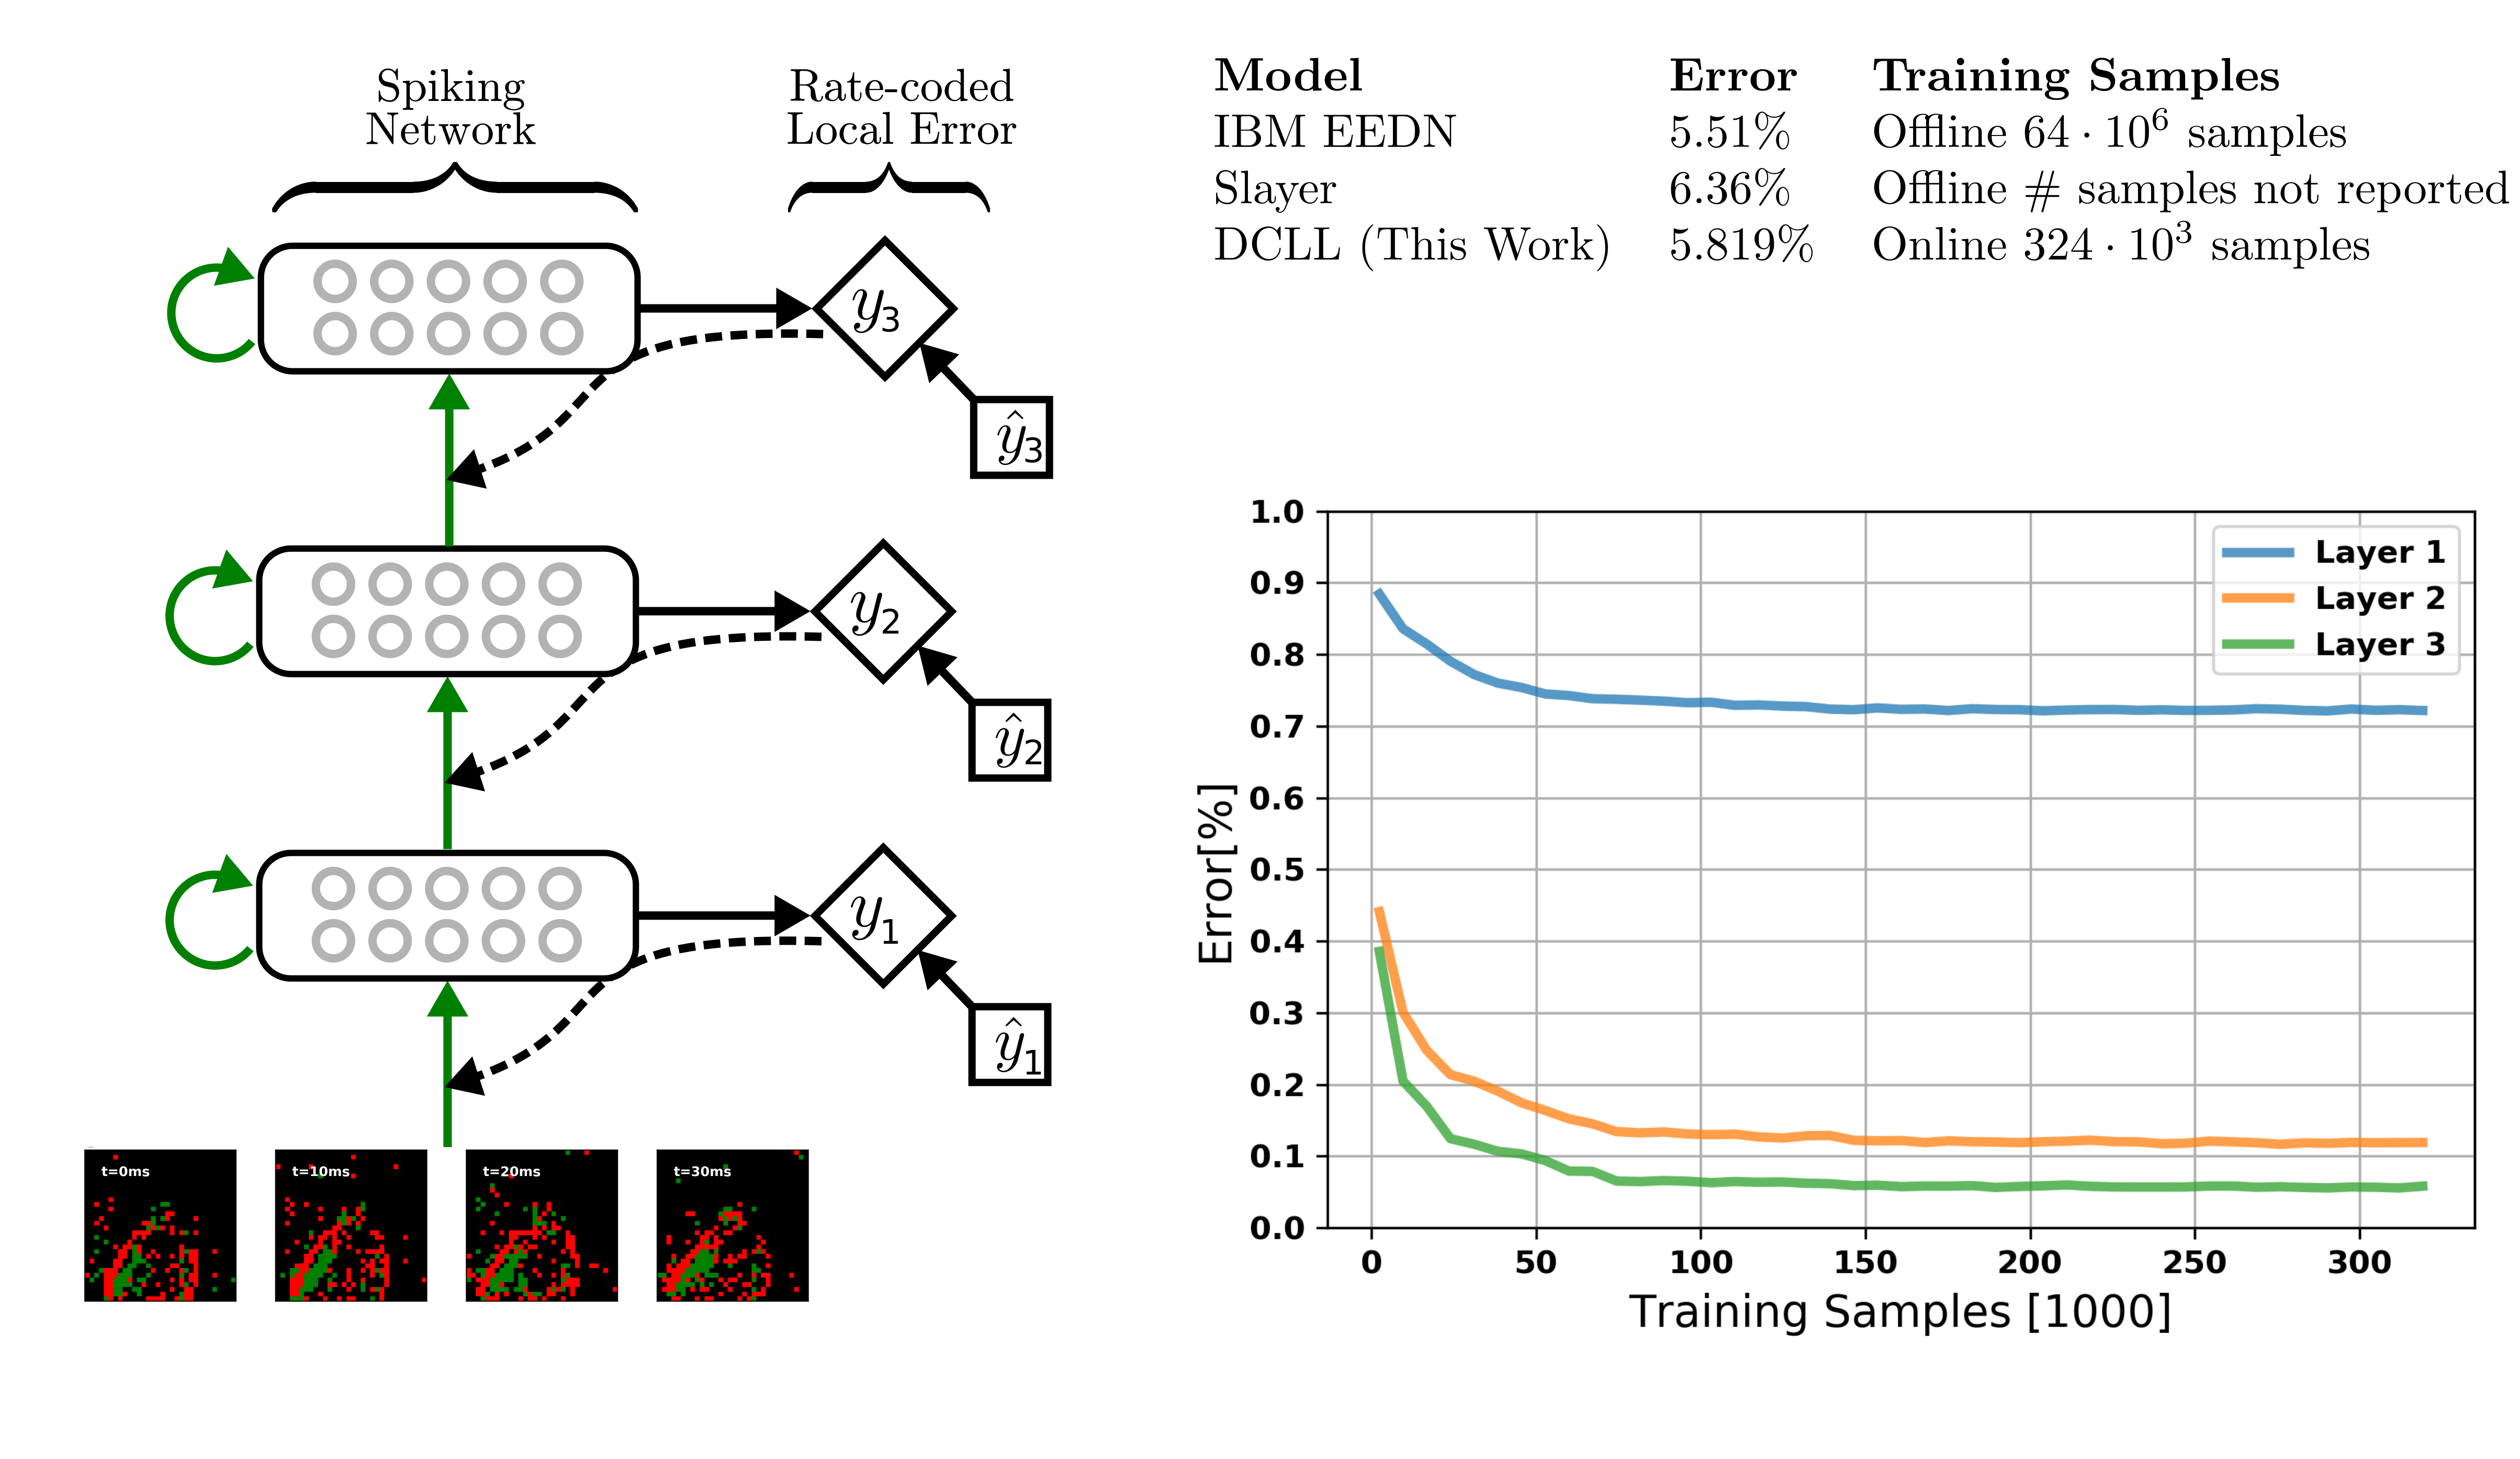
\includegraphics[height=.2\textheight]{./figures/DCLL_illustration.png}
%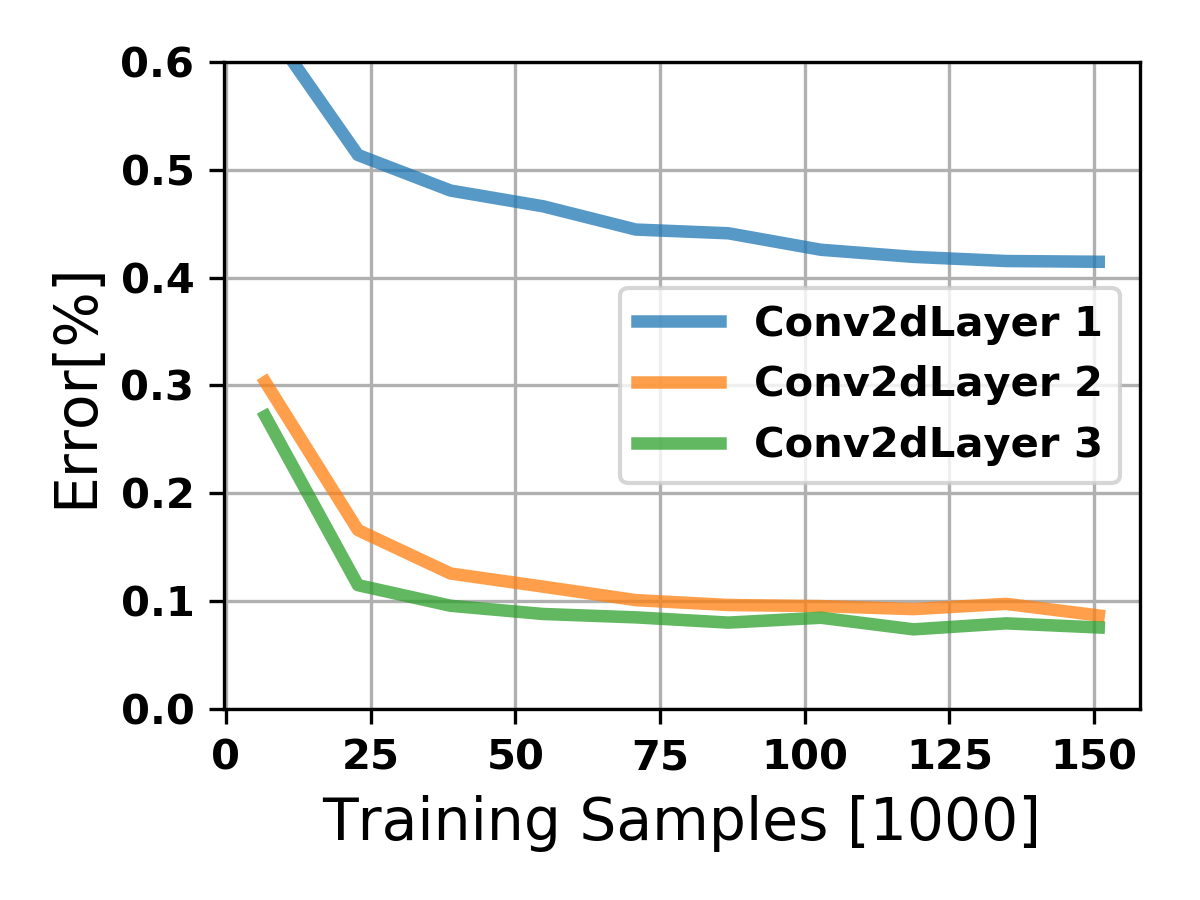
\includegraphics[height=.13\textheight]{./figures/convergence_dvs_gestures_small}
%% \end{center}
%\caption{\label{fig:dcll} Deep Continuous Local Learning (DCLL) with spikes, applied to the DVSGestures dataset. A three layer convolutional spiking neural network is trained with \gls{sg} using local errors generated using fixed random projections to a local classifier. Learning in DCLL scales linearly with the number of neurons thanks to local rate-based cost functions formed by spike-based basis functions. Thanks to the \gls{sg} approach, the plasticity dynamics (dashed line) are synthesized with automatic differentiation under pyTorch. Results here are shown for the DVS Gestures dataset, 11 gestures recorded using a Dynamic Vision Sensor \cite{Amir_etal17_lowpowe}.}
%\end{figure*}




% % Local learning rule Example: SuperSpike
% \paragraph{Stochastic neural networks} \cite{Neftci_etal14_evencont,Neftci17_stocsyna,Neftci_etal17_evenranda}.



% use section* for acknowledgment
% \section*{Acknowledgment}
% This work was partly supported by the Intel Corporation (EN), and the National Science Foundation under grant 1640081 (EN).

% Can use something like this to put references on a page
% by themselves when using endfloat and the captionsoff option.
% \ifCLASSOPTIONcaptionsoff
%   \newpage
% \fi


\bibliographystyle{IEEEtranN}
\bibliography{biblio_unique_alt,fzenke,biblio_hesham}

\section{Author Information}
\textbf{Emre Neftci, UC Irvine (eneftci@uci.edu)}\\
Dr.~Neftci is an assistant professor in the department of Cognitive Sciences and Computer Science at UC Irvine. He received his masters degree in Physics at Ecole Polytechnique Federal de Lausanne (EPFL) and his PhD in Neuroinformatics from the Institute of Neuroinformatics at the university of Zurich and ETH Zurich in neuromorphic engineering. His current research explores the bridges between neuroscience and machine learning, with the focus of theoretical and computational modeling of learning algorithms that are best suited to neuromorphic hardware and non-von Neumann computing architectures.\\

\textbf{Hesham Mostafa, UCSD (hmmostafa@ucsd.edu)}\\
Dr.~Mostafa obtained a master's degree in electrical engineering from the Technical University of Munich in 2010, and a PhD in Neuroinformatics from the Institute of Neuroinformatics at the university of Zurich and ETH Zurich. He is currently a post-doc at the integrated systems neuro-engineering lab at the Institute of Neural Computation at University of California San Diego. His research interests include combining ideas from machine learning and computational neuroscience for developing biologically-inspired and hardware-efficient learning and optimization algorithms, and physically implementing these algorithms using CMOS and novel device technologies.  \\

\textbf{Friedemann Zenke, University of Oxford (friedemann.zenke@cncb.ox.ac.uk)}\\
Dr.~Zenke is a Sir Henry Wellcome post-doctoral fellow at the University of Oxford.
He studied physics at the University of Bonn, Germany and at the Australian National University in Canberra. He received his PhD in the laboratory of Wulfram Gerstner at the EPFL where he studied the interaction of synaptic and homeostatic plasticity in spiking neural network models. He then joined the laboratory of Surya Ganguli at Stanford University as a post-doctoral fellow where he used machine learning approaches to explore learning and memory formation in biologically inspired neural networks. He currently continues this line of research in Tim Vogels' Lab in Oxford.






% %%%%%%%%%%%%%%%%
% \cleardoublepage


% % SuperSpike blurp
% SuperSpike is a voltage-based three factor learning rule which can be run on-line. Instead of back-propagation through time, SuperSpike uses biologically plausible synaptic eligibility traces to deal with the temporal credit assignment problem. 




% \section{Skype Notes}
% \begin{enumerate}
% \item intro to \glspl{snn}, what they are
% \item \glspl{snn}, why is it hard.
% \item Comparison/bridge between artificial neural networks. (table) comparisons with random recurrent neural network.
% \item Bottom-up versus top-down / normative.
% \item Surrogate gradient
% \item What sets us apart from Clopath: learning with hidden units. Layered structure. (Gutig also works on simple, single layer networks). Gradient-based learning. Networks that learn from data and structure and generalize from it.
% \item Machine learning frameworks are great. 
% \item Solve credit assignment problem in space and time.
% \item Surrogate-gradient-based (coin a word?)
% \item Local classifier (spiking version)
% \item Tricks of the trade. Regularization, initialization.
% \item Different types of cost functions. eg we don't care about precise spike timing for classification. How to benchmark.
% \item tasks that SNN excel at is different.
% \item recurrent neural network (?)
% \item Boltzmann machines (?)
% \item Spiking VAE (?)
% \item Training networks on-line. forward in time.
% \end{enumerate}



\end{document}
